\chapter{Vliv odchylek v parametrech na přesnost modelu}

Pro vytvoření modelu spotřeby elektrické energie průmyslového robota je potřeba identifikovat mnoho neznámých parametrů. V případě robota KUKA KR5 Arc se jedná o celkem 54 neznámých parametrů. Ne všechny parametry ale ovlivňují dynamiku robota a s ní spojenou spotřebu elektrické energie stejně. Některé parametry mají mnohem větší vliv než jiné. Pro vytvoření co nejpřesnějšího modelu je proto vhodné tyto parametry identifikovat co nejpřesněji. 

V této sekci je provedena analýza vlivu odchylek v jednotlivých identifikovaných parametrech na přesnost modelu. Dynamický model robota je velmi nelineární. Proto není pro analýzu odchylek parametrů možné použít žádnou z lineárních metod, jako je například určení přenosu ze změny parametru na výstupní výkon nebo simulace systému s jednoduchým zvětšením/zmenšením parametrů. 

Z tohoto důvodu je analýza vlivu odchylek v hodnotách parametrů na přesnost energetického modelu robotu provedena použitím metody Monte Carlo. 

\section{Metoda Monte Carlo}

Metody Monte Carlo jsou založeny na vykonání mnoha opakovaných experimentů nebo simulací s náhodně generovanými vstupními parametry za účelem získání numerických výsledků [\cite{monte_carlo_ref}]. Obdrženou sadu výsledků je poté možné analyzovat analytickými nebo stochastickými metodami. Základní myšlenkou metod Monte Carlo je použití nahodilosti k řešení problémů, které mohou být v principu deterministické.

Tyto metody jsou používány k řešení problémů, u kterých je obtížné nebo dokonce nemožné požít některou z analytických metod. Nejčastěji jsou tyto metody používány pro simulace systémů s mnoha stupni volnosti (kapaliny, systémy s rozprostřenými parametry, propojené systémy), výpočet vícerozměrných určitých integrálů, vyhodnocování rizik v ekonomii a mnoho dalších. 

Analýza vlivu odchylek v identifikovaných parametrech pomocí metody Monte Carlo byla provedena tak, že ke každému z identifikovaných parametrů $P_i$ byla náhodně přičtena hodnota z rozsahu $p \in [-P_i,P_i]$, se kterou byla provedena simulace a vypočítaná střední odchylka mezi simulací a změřenými průběhy. Pro každý parametr bylo takto provedeno 200 simulací, pokaždé s náhodně vygenerovanou hodnotou. Ostatní hodnoty parametrů zůstaly nezměněné. 

Po vykonání simulací pro všechny parametry bylo vyhodnoceno, při jakých odchylkách parametrů byl největší rozdíl mezi simulovaným a změřeným průběhem. 

\section{Vyhodnocení}

Vyhodnocené maximální odchylky mezi simulacemi a změřenými průběhy jsou uvedeny v tabulce \ref{tab_odch_parametru}. Hodnoty v tabulce jsou vztaženy ke střední odchylce mezi výkonem vypočítaným pomocí identifikovaného modelu a určeným pomocí měření proudů (viz sekce \ref{dosaz_presnost_sec}). Hodnoty udávají, o kolik se zvýší odchylka ve wattech mezi modelem a měřením vůči původnímu identifikovanému modelu.

\begin{table}[htbp]
  \centering
  \caption{Tabulka maximálních dosažených odchylek vzhledem k odchylkám v parametrech}
    \begin{tabular}{c|cccccccccc}
    \multicolumn{1}{c|}{Osa} & \multicolumn{1}{c}{$I_{xx}$} & \multicolumn{1}{c}{$I_{yy}$} & \multicolumn{1}{c}{$I_{zz}$} & \multicolumn{1}{c}{$d_x$} & \multicolumn{1}{c}{$d_y$} & \multicolumn{1}{c}{$d_z$} & \multicolumn{1}{c}{$m$} & \multicolumn{1}{c}{$f_v$} & \multicolumn{1}{c}{$f_c$} \\
    \hline
    1  & 0     & 0     & 0.349 & 0     & 0     & 0     & 0     & 18.960 & 0.612 \\
    2  & 0.004 & 0.046 & 0.319 & 1.016 & 0.103 & 0     & 0.022 & 17.824 & 0.506 \\
    3  & 0.003 & 0.171 & 0.726 & 2.320 & 0.824 & 0.087 & 8.202 &  0.568 & 0.053 \\
    4  & 0.811 & 0.043 & 0.041 & 0.586 & 0.055 & 0.047 & 7.963 &  0.094 & 0.002 \\
    5  & 0.033 & 0.018 & 0.029 & 0.427 & 0.004 & 0.044 & 1.394 &  0.078 & 0.021 \\
    6  & 0.065 & 0.027 & 0.002 & 0     & 0     & 0.016 & 0.250 &  0     & 0     \\
    \end{tabular}%
  \label{tab_odch_parametru}%
\end{table}%

Z hodnot v tabulce je možné vypozorovat, že největší vliv na přesnost modelu mají koeficienty viskózního tření ($f_v$) osy 1 a 2 a hmotnosti ramen ($m$) os 3 a 4. Na obrázcích \ref{vliv_odch_1} až \ref{vliv_odch_4} jsou znázorněny vlivy jednotlivých odchylek těchto parametrů na celkovou odchylku modelu vůči měření. Na svislé ose je odchylka, o kterou se zvýší střední odchylka modelu vůči měření v závislosti na změně parametru. Na vodorovné ose je pak odchylka v identifikovaném parametru. 

\begin{figure}[h]
    \centering
    \begin{subfigure}[b]{1\textwidth}
        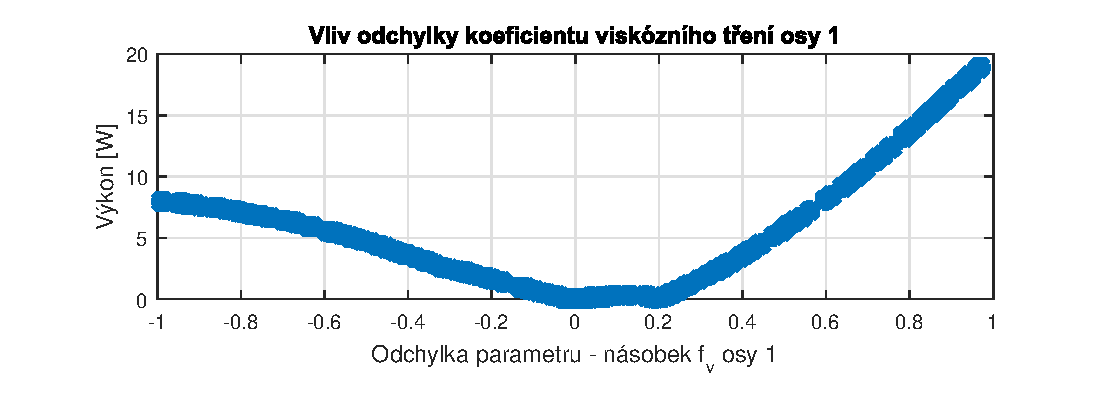
\includegraphics[width=\textwidth]{vliv_odch_osa1_fv}
        \caption{Koeficient viskózního tření osy 1}
        \label{vliv_odch_1}
    \end{subfigure}
    \begin{subfigure}[b]{1\textwidth}
        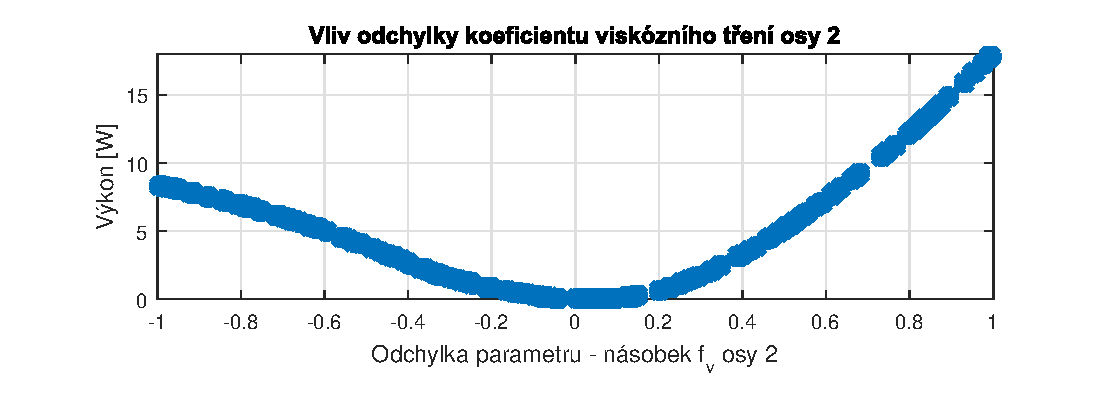
\includegraphics[width=\textwidth]{vliv_odch_osa2_fv}
        \caption{Koeficient viskózního tření osy 2}
        \label{vliv_odch_2}
    \end{subfigure}
    \begin{subfigure}[b]{1\textwidth}
        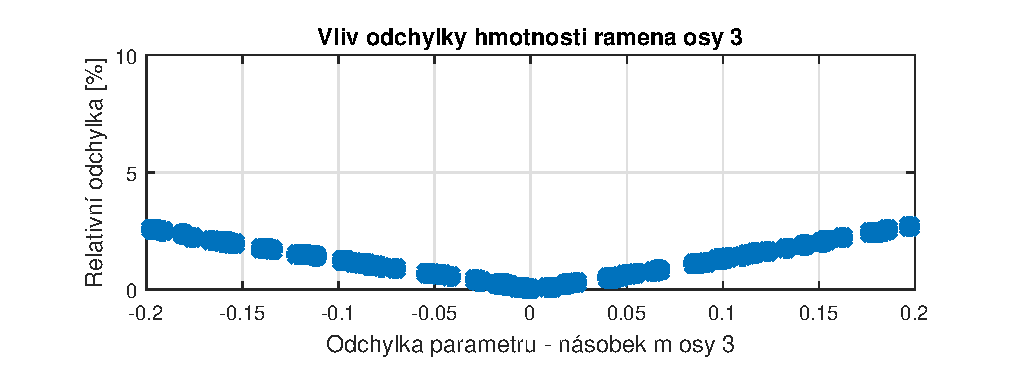
\includegraphics[width=\textwidth]{vliv_odch_osa3_m}
        \caption{Hmotnost osy 3}
        \label{vliv_odch_3}
    \end{subfigure}
    \begin{subfigure}[b]{1\textwidth}
        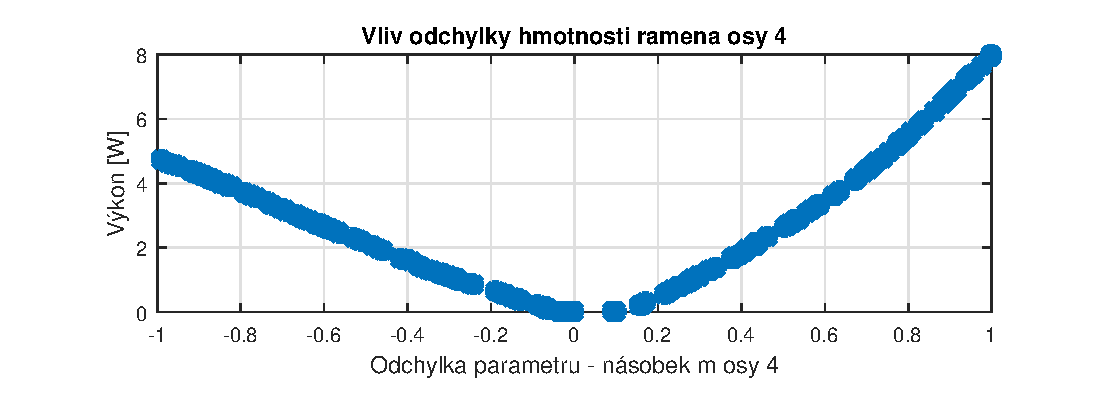
\includegraphics[width=\textwidth]{vliv_odch_osa4_m}
        \caption{Hmotnost osy 4}
        \label{vliv_odch_4}
    \end{subfigure}
    \caption{Vliv odchylek vybraných parametrů na přesnost modelu}
\end{figure} 

\clearpage

Z obrázků je patrné, že metoda identifikace parametrů (viz sekce \ref{z_rovnic_sec}) nalezla optimální řešení, protože zvýšení i snížení identifikovaných parametrů vede na větší střední odchylku mezi modelem a měřením. 

Největší vliv na přesnost modelu mají tedy koeficienty tření, hmotnosti a polohy těžišť prvních tří os. Z toho důvodu je vhodné identifikovat tyto parametry co nejpřesněji.   